
% This LaTeX was auto-generated from an M-file by MATLAB.
% To make changes, update the M-file and republish this document.

\documentclass{article}

\author{Michael Graczyk}




\usepackage{fullpage}
\usepackage{color,graphicx}
\usepackage{amsmath, amsthm, amsfonts,amsbsy} 
\usepackage{listings}
\usepackage{float}

% Macro Definitions
\newcommand{\RR}{\mathbb{R}}

\sloppy
\definecolor{lightgray}{gray}{0.5}
\setlength{\parindent}{0pt}

\begin{document}
	

	\lstset{ %
		language=MATLAB,                % choose the language of the code
		basicstyle=\footnotesize,       % the size of the fonts that are used for the code
		numbers=left,                   % where to put the line-numbers
		numberstyle=\footnotesize,      % the size of the fonts that are used for the line-numbers
		stepnumber=1,                   % the step between two line-numbers. If it is 1 each line will be numbered
		showspaces=false,               % show spaces adding particular underscores
		showstringspaces=false,         % underline spaces within strings
		showtabs=false,                 % show tabs within strings adding particular underscores
		frame=single,           % adds a frame around the code
		tabsize=3,          % sets default tabsize to 2 spaces
		captionpos=b,           % sets the caption-position to bottom
		breaklines=true,        % sets automatic line breaking
		breakatwhitespace=false,    % sets if automatic breaks should only happen at whitespace
		escapeinside={\%*}{*)}          % if you want to add a comment within your code
	}
	
    \begin{figure}[H]
   \caption{Matlab Code}
   \centering
\begin{lstlisting}
% Read in sample rain file and clip a short amount
[rain_sound, Fs, Nbits] = wavread('rain.wav');
rain_sound = rain_sound(2000000:2500000,:);
white_noise = wgn(100000,1, -22);

figure(1);
subplot(2,2,1);
spectrogram(rain_sound(200000:300000,1), hamming(100), 0, 512, Fs);
title('Rain Spectrogram');

subplot(2,2,2);
spectrogram(white_noise, hamming(100), 0, 512, Fs);
title('WGN Spectrogram');

% Make some phase noise
a = zeros(1,100);
a(1) = 1;
for ii = 2:100
a(ii) = (ii - 2.5) * a(ii-1) / (ii-1);
end
theta = filter(1,a,white_noise);
phase_noise = exp(1.0i*theta);
subplot(2,2,3);
spectrogram(phase_noise, hamming(100), 0, 512, Fs);
title('Phase Noise');

% Read some Brown Noise
[brown_noise FsB, ~] = wavread('brownnoise.wav');
brown_noise = brown_noise(1:100000);
subplot(2,2,4);
spectrogram(brown_noise, hamming(100), 0, 512, Fs);
title('Brown Noise');
\end{lstlisting}
\end{figure}

\begin{center}
	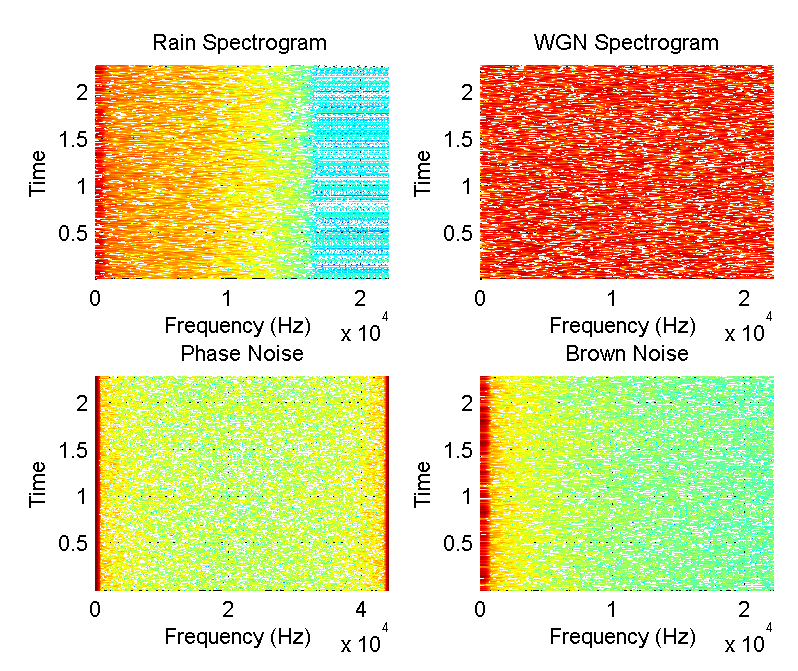
\includegraphics [width=6in]{PropEx_01.eps}
\end{center}



\end{document}
    
